% !TEX root=../main.tex

\subsection{Example}
\label{sec:example}

Now that we have studied all editor types, the core task combinators, and some derived forms,
we develop an example program to demonstrate the capabilities of \TOPHAT.
The example is a small flight booking system.
We demonstrate communication on all three levels: with the environment, alongside control flow, and across it.
Also, we show synchronisation, input validation, and the uses of different kinds of editors.

% \subsection[sub:flight-example]{Flight booking}

The requirements of our flight booking application are as follows:
\begin{itemize}
  \item Users have to enter a list of passengers for which to book tickets.
  \item At least one of these passengers has to be an adult.
  \item After a valid list of passengers has been entered, users have to pick seats.
  \item Only free seats may be picked.
  \item Every passenger must have exactly one seat.
  \item Multiple users should be able to book tickets at the same time.
\end{itemize}

For this example we assume that the host language has lists and four functions over them:
\var{all}, \var{any}, \var{intersect}, and \var{difference}.
The functions \var{all} and \var{any} check if all or any elements in a list satisfy a given predicate.
The functions \var{intersect} and \var{difference} compute the set-intersection and set-difference of two lists.
For brevity, we omit the type annotations of variable bindings.

\begin{example}{Flight booking}
  \label{exm:flight-booking}
  % \todo{Fix example}
  We start off by defining some type aliases.
  A passenger is a pair with name and age.
  A seat is a pair with a row number and a seat letter.
  \begin{TASK}[]
    type Passenger = String * Int
    type Seat = Int * String
  \end{TASK}

  Now we develop our workflow in a top-down fashion.
  The main task starts three \var{bookFlight} tasks,
  which could be performed by three different users in parallel.
  Choosing seats requires reading and updating shared information.
  The list of free seats is stored in a reference,
  which is passed to all instances of \var{bookFlight}.
  \begin{TASK}[emph={free}]
    share [ {1,"A"}, {1,"B"}, {1,"C"}, ... ] >>= do free.
    bookFlight free <&> bookFlight free <&> bookFlight free
  \end{TASK}

  Our flight booking starts with an interactive task \var{enter (List Passenger)}, where users can enter a list of passengers.
  A task $\Enter \tau$ is an empty editor that asks for a value of the given type $\tau$.
  \begin{TASK}[emph={pgrs,free}]
    let bookFlight = do free. enter (List Passenger) >>? do pgrs.
      if allValid pgrs then chooseSeats pgrs free else fail
  \end{TASK}
  When users have entered a valid list of passengers, the step after \var{>>?} becomes enabled,
  and they can proceed to picking seats.
  In case of an invalid list of passengers,
  the step is guarded by the failing task~\var{fail}.


  Passengers are valid if their name is not empty and their age is at least $0$.
  Lists of passengers are valid if each passenger is valid, and at least one of the passengers is an adult.
  \begin{TASK}[emph={name,age,seats,pgrs,free}]
    let allValid = do pgrs. all valid pgrs && any adult pgrs
    let valid = do {name, age}. not (name == "") && age >= 0
    let adult = do {_, age}. age >= 18
  \end{TASK}

  A selection of seats is correct if every entered seat is free.
  \begin{TASK}[emph={name,age,seats,free,pgrs,freeSeats}]
    let chooseSeats = do pgrs. do free. enter (List Seat) >>? do seats.
      if correct seats free && length pgrs == length seats
        then confirmBooking pgrs seats free else fail
    let correct = do seats. do free. watch free >>= do freeSeats.
      intersect seats freeSeats == seats
  \end{TASK}

  The function \var{confirmBooking} removes the selected seats from the shared list of free seats,
  and displays the end result using a read-only editor.
  \begin{TASK}[emph={name,age,seats,pgrs,free}]
    let confirmBooking = do pgrs. do seats. do free.
      free ::= difference seats >>= do  _.
      view {pgrs, seats}
  \end{TASK}
  % It uses a function \var{difference}, which removes all elements from the second list from the first list.

  \begin{figure}
    \label{fig:flight-booking}
    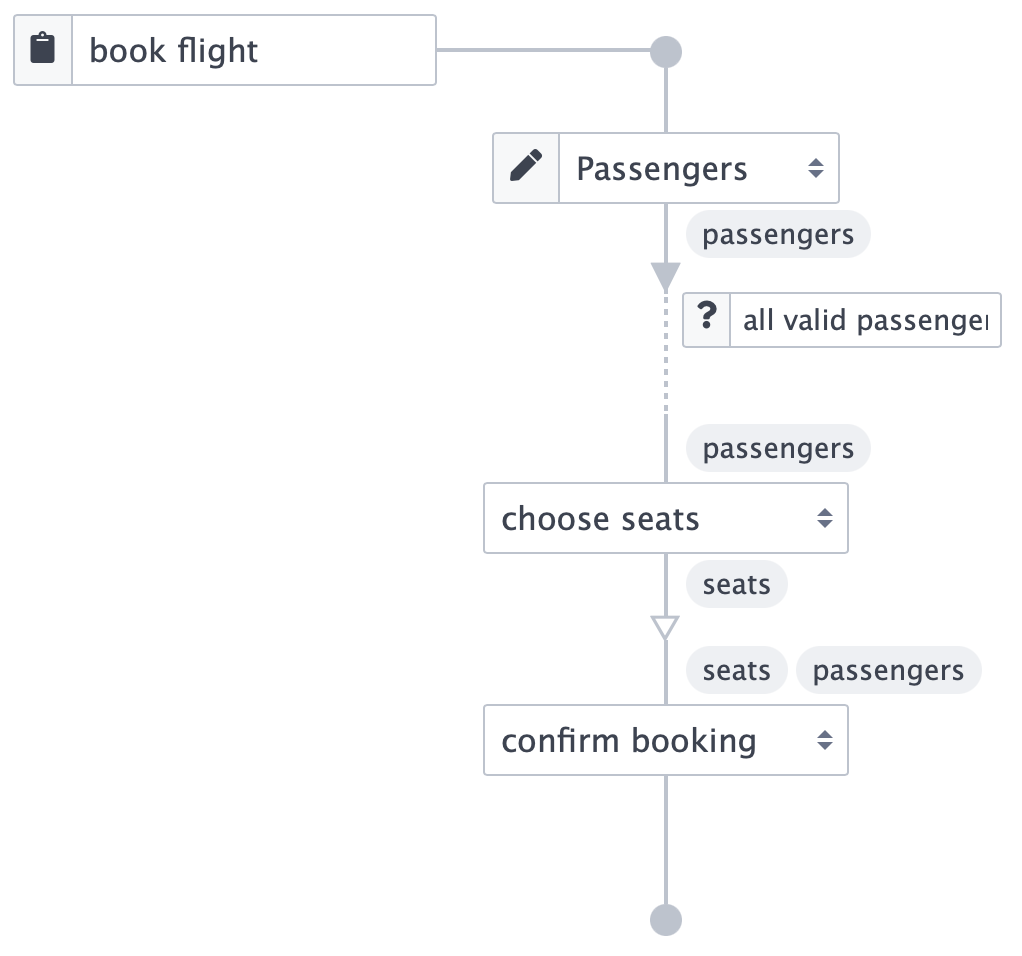
\includegraphics[width=\columnwidth]{figures/flight-booking.png}
    \caption{Running web application of the flight booking example using an elaboration into \ITASKS.}
    %  It shows three users booking a flight simultaneously.
    %  The first user entered name and age and continued picking seats.
    %  The second is entering details of two passengers.
    %  The ages are not filled in, therefore the \var{Continue} button is disabled.
    %  The message bubble shows that the \var{age} field only accepts integer values.
    %  The third user finished a booking,
    %  therefore, the first user can not pick seats \smallcaps{1b} and \smallcaps{1c} any more.}
  \end{figure}

  We can run this program by translating above \TOPHAT\ code to \ITASKS.
  % \cref{app:itasks} gives an overview of equivalent constructs in both systems.
  A screenshot of the resulting web application is shown in \cref{fig:flight-booking}.

  All instances of the \var{bookFlight} task have access to the shared list of free seats.
  Rewriting the example in a language without references would not only be cumbersome,
  % obfuscating the code with explicit threading of state,
  but it would be impossible to model the parallel execution of three \var{bookFlight} tasks.
  It is not known upfront which task will finish first,
  and thus it is not possible to thread the free seat list itself between the parallel tasks.
\end{example}

% \begin{TASK}[emph={passengers,chosen,free}]
%   let main =
%     share [(1, 'A'), (1, 'B'), (2, 'A'), (2, 'B'), ...] >>= do free.
%     watch free <&> >&<$_\text{\var{book \emph{free}}}$ []

%   let book = do free.
%     enter List Passenger >>= do passengers.
%       all valid passengers |->
%         choose_seats passengers free >>= do chosen.
%         confirm_booking passengers chosen >>= do _.
%         assert length passengers == length chosen
%         assert unique chosen
%         assert chosen /< free

%   let choose_seats = do passengers. do free.
%     (watch free <&> enter Seats) >>= do (free, chosen).
%     intersect chosen free /\ length passengers == length chosen
%       |-> confirm_booking passengers chosen free

%   let confirm_booking = do passengers. do chosen. do free.
%     free ::= difference chosen
%     view (passengers, chosen)
% \end{TASK}

%   % allValid :: Passengers -> Bool
%   % allValid ps = all isValid ps && any isAdult ps

%   % isValid :: Passenger -> Bool
%   % isValid (n, a) = n /= "" && a >= 0

%   % isAdult :: Passenger -> Bool
%   % isAdult (_, a) = a >= 18

%   % isCorrect :: Seats -> Seats -> Bool
%   % isCorrect ss fs = do
%   %   List.intersect ss fs == ss

% \begin{TASK}[emph={passengers,seats,free}]
%   let book_flight = do free.
%     enter List Passenger >>= do passengers.
%       all valid passengers |->
%         choose_seats passengers >>= do seats.
%         confirm_booking passengers seats
%         assert length passengers == length seats
%         assert unique seats
%         assert seats /< free
% \end{TASK}

% \begin{TASK}[emph={passengers,seats,free}]
%   book_flight free <&> book_flight free
% \end{TASK}

% \begin{TASK}[emph={passengers,seats,free}]
%   let main =
%     book_flight free
%           <&>
%     book_flight free
%           <&>
%     book_flight free
%           <&>
%            $\vdots$
% \end{TASK}

% \begin{TASK}[emph={passengers,seats,free}]
%   let main =
%     >&<$_\text{\var{book\_flight \emph{free}}}$ []
% \end{TASK}
% \begin{TASK}[emph={passengers,seats,free}]
%   let main =
%     >&<$_\text{\var{book\_flight \emph{free}}}$ [book_flight free]
% \end{TASK}
% \begin{TASK}[emph={passengers,seats,free}]
%   let main =
%     >&<$_\text{\var{book\_flight \emph{free}}}$ [choose_seats ..., book_flight free]
% \end{TASK}
% \begin{TASK}[emph={passengers,seats,free}]
%   let main =
%     >&<$_\text{\var{book\_flight \emph{free}}}$ [choose_seats ...]
% \end{TASK}